\documentclass[12pt,a4paper]{article}%
\usepackage{amsthm}
\usepackage{amsmath}%
\usepackage{amsfonts}%
\usepackage{amssymb}%
\usepackage{graphicx}
\usepackage{float}
\usepackage[T2A]{fontenc}
\usepackage[utf8]{inputenc}
\usepackage[english,russian]{babel}
%-------------------------------------------
\setlength{\textwidth}{7.0in}
\setlength{\oddsidemargin}{-0.35in}
\setlength{\topmargin}{-0.5in}
\setlength{\textheight}{9.0in}
\setlength{\parindent}{0.3in}

\newtheorem{theorem}{Theorem}
\newtheorem{task}[theorem]{Задача}
\addto\captionsrussian{\renewcommand*{\proofname}{Решение}}


\newcommand{\abovemath}[2]{\ensuremath{\stackrel{\text{#1}}{#2}}}
\newcommand{\aboveeq}[1]{\abovemath{#1}{=}}
\newcommand\bydef{\aboveeq{def}}
\begin{document}


\begin{flushright}
\textbf{Мирончик Павел \\
\today}
\end{flushright}

\begin{center}
\textbf{Формальные языки\\
HW02} \\
\end{center}

\task{
  Привести полный минимальный детерминированный конечный автомат для следующих языков

  \begin{enumerate}
    \item $\{\omega \in \{0, 1, \dots, 9\}^* \mid \omega \text{ делится нацело на } 5 \}$
    \begin{proof}{}
        В первом задании я счел, что пустая последовательность не является допустимой. 
        \begin{figure}[h!]
	    \centering
	    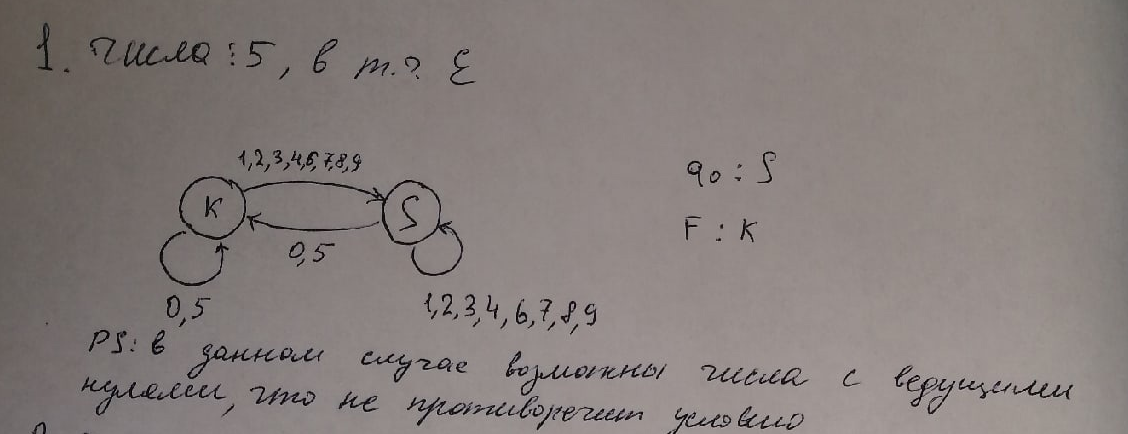
\includegraphics[width=0.8\linewidth]{proof1.png}
        \end{figure}
    \end{proof}

    \item Язык положительных чисел с плавающей точкой. Целая часть может отсутствовать, дробная часть может отсутствовать, но не одновременно. Перед точкой может не быть ничего. Лидирующих нулей быть не должно
    \begin{itemize}
      \item $123.45, .45, 123$ -- числа
      \item $\varepsilon, ., abc, 123., 1.2.3.4, 007$ -- не числа
    \end{itemize}
    \begin{proof}{} \hfill
        \begin{figure}[h!]
	    \centering
	    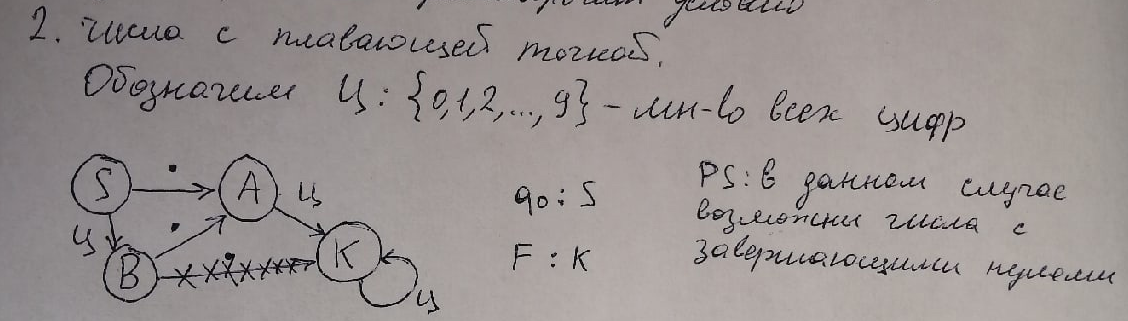
\includegraphics[width=0.8\linewidth]{proof2.png}
        \end{figure}
    \end{proof}

    \newpage
    \item $\{\omega \in \{a, b\}^* \mid |\omega|_a \leq 3, |\omega|_b > 2\}$
    %\hfill
    \begin{proof}{} \hfill
        \begin{figure}[h]
	    \centering
	    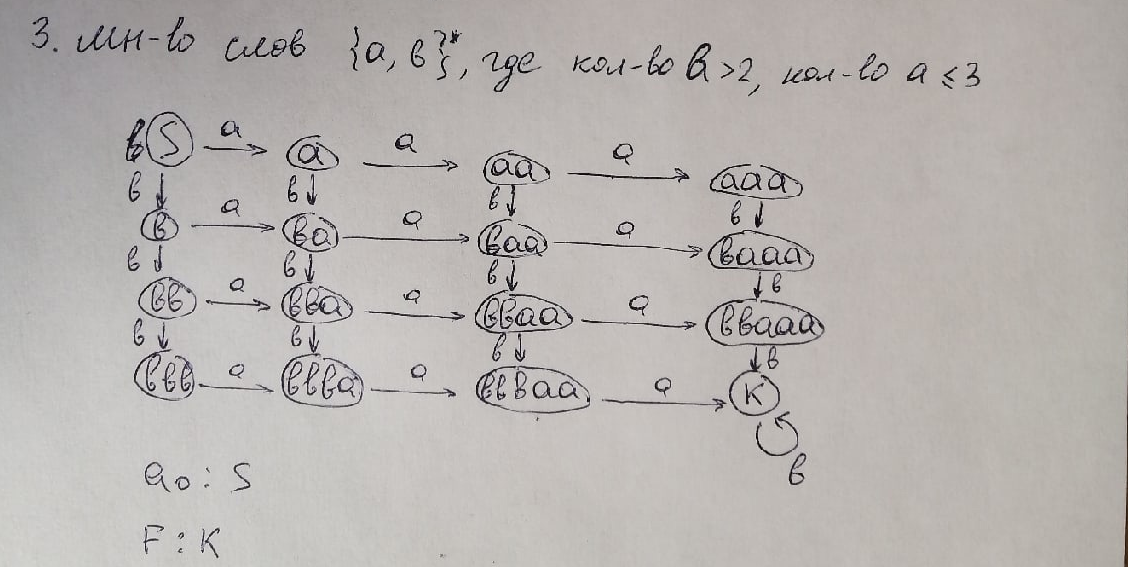
\includegraphics[width=0.8\linewidth]{proof3.png}
        \end{figure}
    \end{proof}
  \end{enumerate}
}

\end{document}